\chapter{Implementierung}
\section{Implementierung der Schnittstelle}
%Warum wird nutzt die ThalesApi gRPC?
Die ThalesApi wird verwendet um die Sensordaten der Test Sceneie weiterzuleiten.
Die ThalesApi gRPC verwendet das Protocol Buffers (protobuf) Datenformat, das binär kodiert ist und daher effizienter als JSON oder XML ist. Dies führt zu schnellerer Datenübertragung und geringerem Ressourcenverbrauch, was in Spielen und anderen Unity-Anwendungen wichtig ist.\\
Das gRPC Protokocol welches die ThalesApi verwendet bietet Unterstützung für eine Vielzahl von Programmiersprachen, darunter C\#, was die Integration in Unity erleichtert. Dies ermöglicht es, Client-Server-Kommunikation nahtlos zwischen Unity und anderen Serveranwendungen in verschiedenen Sprachen herzustellen. Die Clients können in vielen Sprachen geschrieben werden. Im DSM Projekt wird ein C++ CLient verwendet.\\
Mit gRPC können Sie starke Typisierung für Ihre Dienstaufrufe verwenden. Dies bedeutet, dass Sie spezifische Methodenaufrufe mit stark typisierten Eingabe- und Ausgabeparametern definieren können, was die Entwicklung und Wartung Ihrer Anwendung erleichtert.\\
gRPC unterstützt bidirektionale Streaming-Kommunikation, was bedeutet, dass sowohl der Client als auch der Server Daten an den anderen senden können, ohne auf eine Anfrage des anderen zu warten. Dies ist besonders nützlich für Multiplayer-Spiele und Echtzeit-Anwendungen.\\
gRPC bietet Tools zur automatischen Codegenerierung, um Client- und Serverstubs sowie die erforderlichen Datenklassen basierend auf Ihren Protobuf-Definitionen zu erstellen. Dies vereinfacht die Entwicklung und verhindert Fehler durch manuelle Codeerstellung. Dies wird vorallem für die CustumApi genutzt, um beliebige Variablen zuübertragen.\\
%An meinem Tutorial orientieren
Die ThalesApi basiert auf gRPC. Die ThalesApi erstellt einen gRPC Server dessen Services von einem Client abgerufen werden.  

%wie funktioniert die ThalesApi?
Sobald die ThalesApi der Scene hinzugefügt wird können die Sensordaten mit dem Client abgerfagt werden.

%Warum muss ein Autostepper verwendet werden?
%Wie wird der Sensor in Konfiguriet

%Wann wird diese Aktiv?
\subsection{Übertragung von den Sensordaten}
%Wie wurde es nochmal genau gemacht?
Die Sensor daten werden über den Client abgerufen.

\begin{lstlisting}[caption=Sample Code Listing C++, label={lst:listing-cpp}, language=C++]
int main(int argc, char** argv) {
    auto consoleOutput = std::make_shared<sick::dsm::consumers::ConsoleOutputConsumer>();
    auto slaveProxy0 = std::make_shared<sick::dsm::proxies::SlaveProxy>("127.0.0.1", 5555, 6555);
    slaveProxy0->setSendImmediately(true).setMaxSlices(1).setSliceBeamCount(2200).setMtuSize(1460).setIndex(0).setIdentifier({127, 0, 0, 1, 0x15, 0xb3, 0, 0}).initialise();
    auto slaveProxy1 = std::make_shared<sick::dsm::proxies::SlaveProxy>("127.0.0.1", 5556, 6556);
    slaveProxy1->setSendImmediately(true).setMaxSlices(1).setSliceBeamCount(2200).setMtuSize(1460).setIndex(0).setIdentifier({127, 0, 0, 1, 0x15, 0xb4, 0, 0}).initialise();
    auto slaveProxy2 = std::make_shared<sick::dsm::proxies::SlaveProxy>("127.0.0.1", 5557, 6557);
    slaveProxy2->setSendImmediately(true).setMaxSlices(1).setSliceBeamCount(2200).setMtuSize(1460).setIndex(0).setIdentifier({127, 0, 0, 1, 0x15, 0xb5, 0, 0}).initialise();
    auto slaveProxy3 = std::make_shared<sick::dsm::proxies::SlaveProxy>("127.0.0.1", 5558, 6558);
    slaveProxy3->setSendImmediately(true).setMaxSlices(1).setSliceBeamCount(2200).setMtuSize(1460).setIndex(0).setIdentifier({127, 0, 0, 1, 0x15, 0xb6, 0, 0}).initialise();
    std::string connectionString = "192.168.100.1:30718";
    std::shared_ptr<grpc::Channel> channel = sick::dsm::producers::ThalesGrpcClient::getInstance(connectionString).getChannel();

    std::string scannerObjectPath0 = "BasicVehicle/microScan3-maxRange-Rasterization-0";
    std::string scannerObjectPath1 = "BasicVehicle/microScan3-maxRange-Rasterization-1";
    std::string scannerObjectPath2 = "BasicVehicle/microScan3-maxRange-Rasterization-2";
    std::string scannerObjectPath3 = "BasicVehicle/microScan3-maxRange-Rasterization-3";
    auto scanner0 = std::make_shared<sick::dsm::producers::ThalesScanner>(scannerObjectPath0, channel);
    auto scanner1 = std::make_shared<sick::dsm::producers::ThalesScanner>(scannerObjectPath1, channel);
    auto scanner2 = std::make_shared<sick::dsm::producers::ThalesScanner>(scannerObjectPath2, channel);
    auto scanner3 = std::make_shared<sick::dsm::producers::ThalesScanner>(scannerObjectPath3, channel);
    scanner0->addConsumer(slaveProxy0);
    scanner1->addConsumer(slaveProxy1);
    scanner2->addConsumer(slaveProxy2);
    scanner3->addConsumer(slaveProxy3);

    auto recorder0 = std::make_shared<sick::dsm::consumers::FileRecorder>("recorder0.bin");
    auto recorder1 = std::make_shared<sick::dsm::consumers::FileRecorder>("recorder1.bin");
    auto recorder2 = std::make_shared<sick::dsm::consumers::FileRecorder>("recorder2.bin");
    auto recorder3 = std::make_shared<sick::dsm::consumers::FileRecorder>("recorder3.bin");


    sick::dsm::proxies::MasterProxy masterProxy0(5555, {127, 0, 0, 1, 0x15, 0xb3, 0, 0});
    masterProxy0.addConsumer(recorder0);
    // masterProxy0.addConsumer(consoleOutput);
    masterProxy0.start();

    sick::dsm::proxies::MasterProxy masterProxy1(5556, {127, 0, 0, 1, 0x15, 0xb4, 0, 0});
    masterProxy1.addConsumer(recorder1);
    // masterProxy1.addConsumer(consoleOutput);
    masterProxy1.start();

    sick::dsm::proxies::MasterProxy masterProxy2(5557, {127, 0, 0, 1, 0x15, 0xb5, 0, 0});
    masterProxy2.addConsumer(recorder2);
    // masterProxy2.addConsumer(consoleOutput);
    masterProxy2.start();

    sick::dsm::proxies::MasterProxy masterProxy3(5558, {127, 0, 0, 1, 0x15, 0xb6, 0, 0});
    masterProxy3.addConsumer(recorder3);
    // masterProxy3.addConsumer(consoleOutput);
    masterProxy3.start();

    scanner0->start();
    scanner1->start();
    scanner2->start();
    scanner3->start();

    int counter = 0;
    std::thread t1([&](){
        while (true) {
            scanner0->produce();
            scanner1->produce();
            scanner2->produce();
            scanner3->produce();
            std::this_thread::sleep_for(std::chrono::milliseconds(500));
        }
    });
    std::thread t2([&](){
        while (true) {
            masterProxy0.produce();
            masterProxy1.produce();
            masterProxy2.produce();
            masterProxy3.produce();
            std::this_thread::sleep_for(std::chrono::milliseconds(500));
        }
    });
    t1.join();
    t2.join();
    return 0;
}
\end{lstlisting}
Der Code beginnt mit Include-Deklarationen, die die notwendigen Header-Dateien für die Verwendung von C++-Standardbibliotheksfunktionen und anderen Bibliotheken wie gRPC und der "sick::dsm"-Bibliothek importieren.\\

Im weiteren Verlauf des Codes werden verschiedene Variablen und Objekte deklariert. Dazu gehören Objekte wie consoleOutput, slaveProxy0, slaveProxy1, slaveProxy2, slaveProxy3, channel, scanner0, scanner1, scanner2, scanner3, recorder0, recorder1, recorder2, recorder3, masterProxy0, masterProxy1, masterProxy2 und masterProxy3. Diese Objekte repräsentieren verschiedene Teile der Anwendung, darunter die Kommunikation mit Laserscannern, die Aufzeichnung von Daten und die Verwendung von gRPC für die Kommunikation.\\

Die Slave-Proxies (slaveProxy0, slaveProxy1, slaveProxy2, slaveProxy3) werden konfiguriert, um Verbindungen zu bestimmten IP-Adressen und Ports herzustellen. Diese Proxies werden wahrscheinlich verwendet, um Daten von den Laserscannern zu empfangen und zu verarbeiten.\\

Eine gRPC-Verbindung (channel) zu einer bestimmten IP-Adresse und Port wird erstellt. Dies wird wahrscheinlich für die Kommunikation mit einem entfernten Server verwendet.\\

Es werden Scanner-Objekte (scanner0, scanner1, scanner2, scanner3) erstellt und für die Verarbeitung von Daten aus den Laserscannern konfiguriert. Sie fügen auch Slave-Proxies als Verbraucher hinzu, um die verarbeiteten Daten weiterzuleiten.\\

Recorder-Objekte (recorder0, recorder1, recorder2, recorder3) werden erstellt. Diese Objekte zeichnen Daten in Dateien auf.\\

Master-Proxies (masterProxy0, masterProxy1, masterProxy2, masterProxy3) werden konfiguriert, um Daten von den Slave-Proxies zu empfangen und wahrscheinlich weitere Verarbeitung oder Aufzeichnung durchzuführen.\\

Es werden zwei Threads (t1 und t2) erstellt, die kontinuierlich Daten von Scannern und Master-Proxies produzieren. Diese Threads laufen in einer Endlosschleife und führen die entsprechenden Produktionsschritte aus.\\
%Es wurde eine Subsriction erstellt
%Die Sensordaten werden abgefragt sondern sie sollen alle daten geschickt werden die aufgenommen wurden
%Wie wurde der Client gestalltet?
%Client mit ChatGpt kommentieren lassen

\subsection{Übertragung von Variablen}
%Wie erstellt man eine CustumApi?
%Warum nutzt man die CustumApi?
%Wie wird die CustumApi in Unity verwendet?
%Wo für verwendete die CustumApi?


%\section{AGVs in der virtuellen Umgebung}
\section{Umsetzung der Fahrphysik}
\subsection{Lenkung}
%Wie funktioneriert die Lenkung mit Ackermann winkel
Der Lenk mechanismus wird durch den Ackermannwinkel umgesetzt.
%Warum wurde dieser verwendetet?
Der Ackermannwinkel wird verwendet weil das Äußere Rat und das innere Rad einen anderen Wendekreis. Wenn die beiden Räder den gleichen Einschlagwinkel haben würde das Rad mit der geringeren haftung zum boden den Kontakt zudiesem verlieren.\\
\begin{figure}[htp]
    \centering
    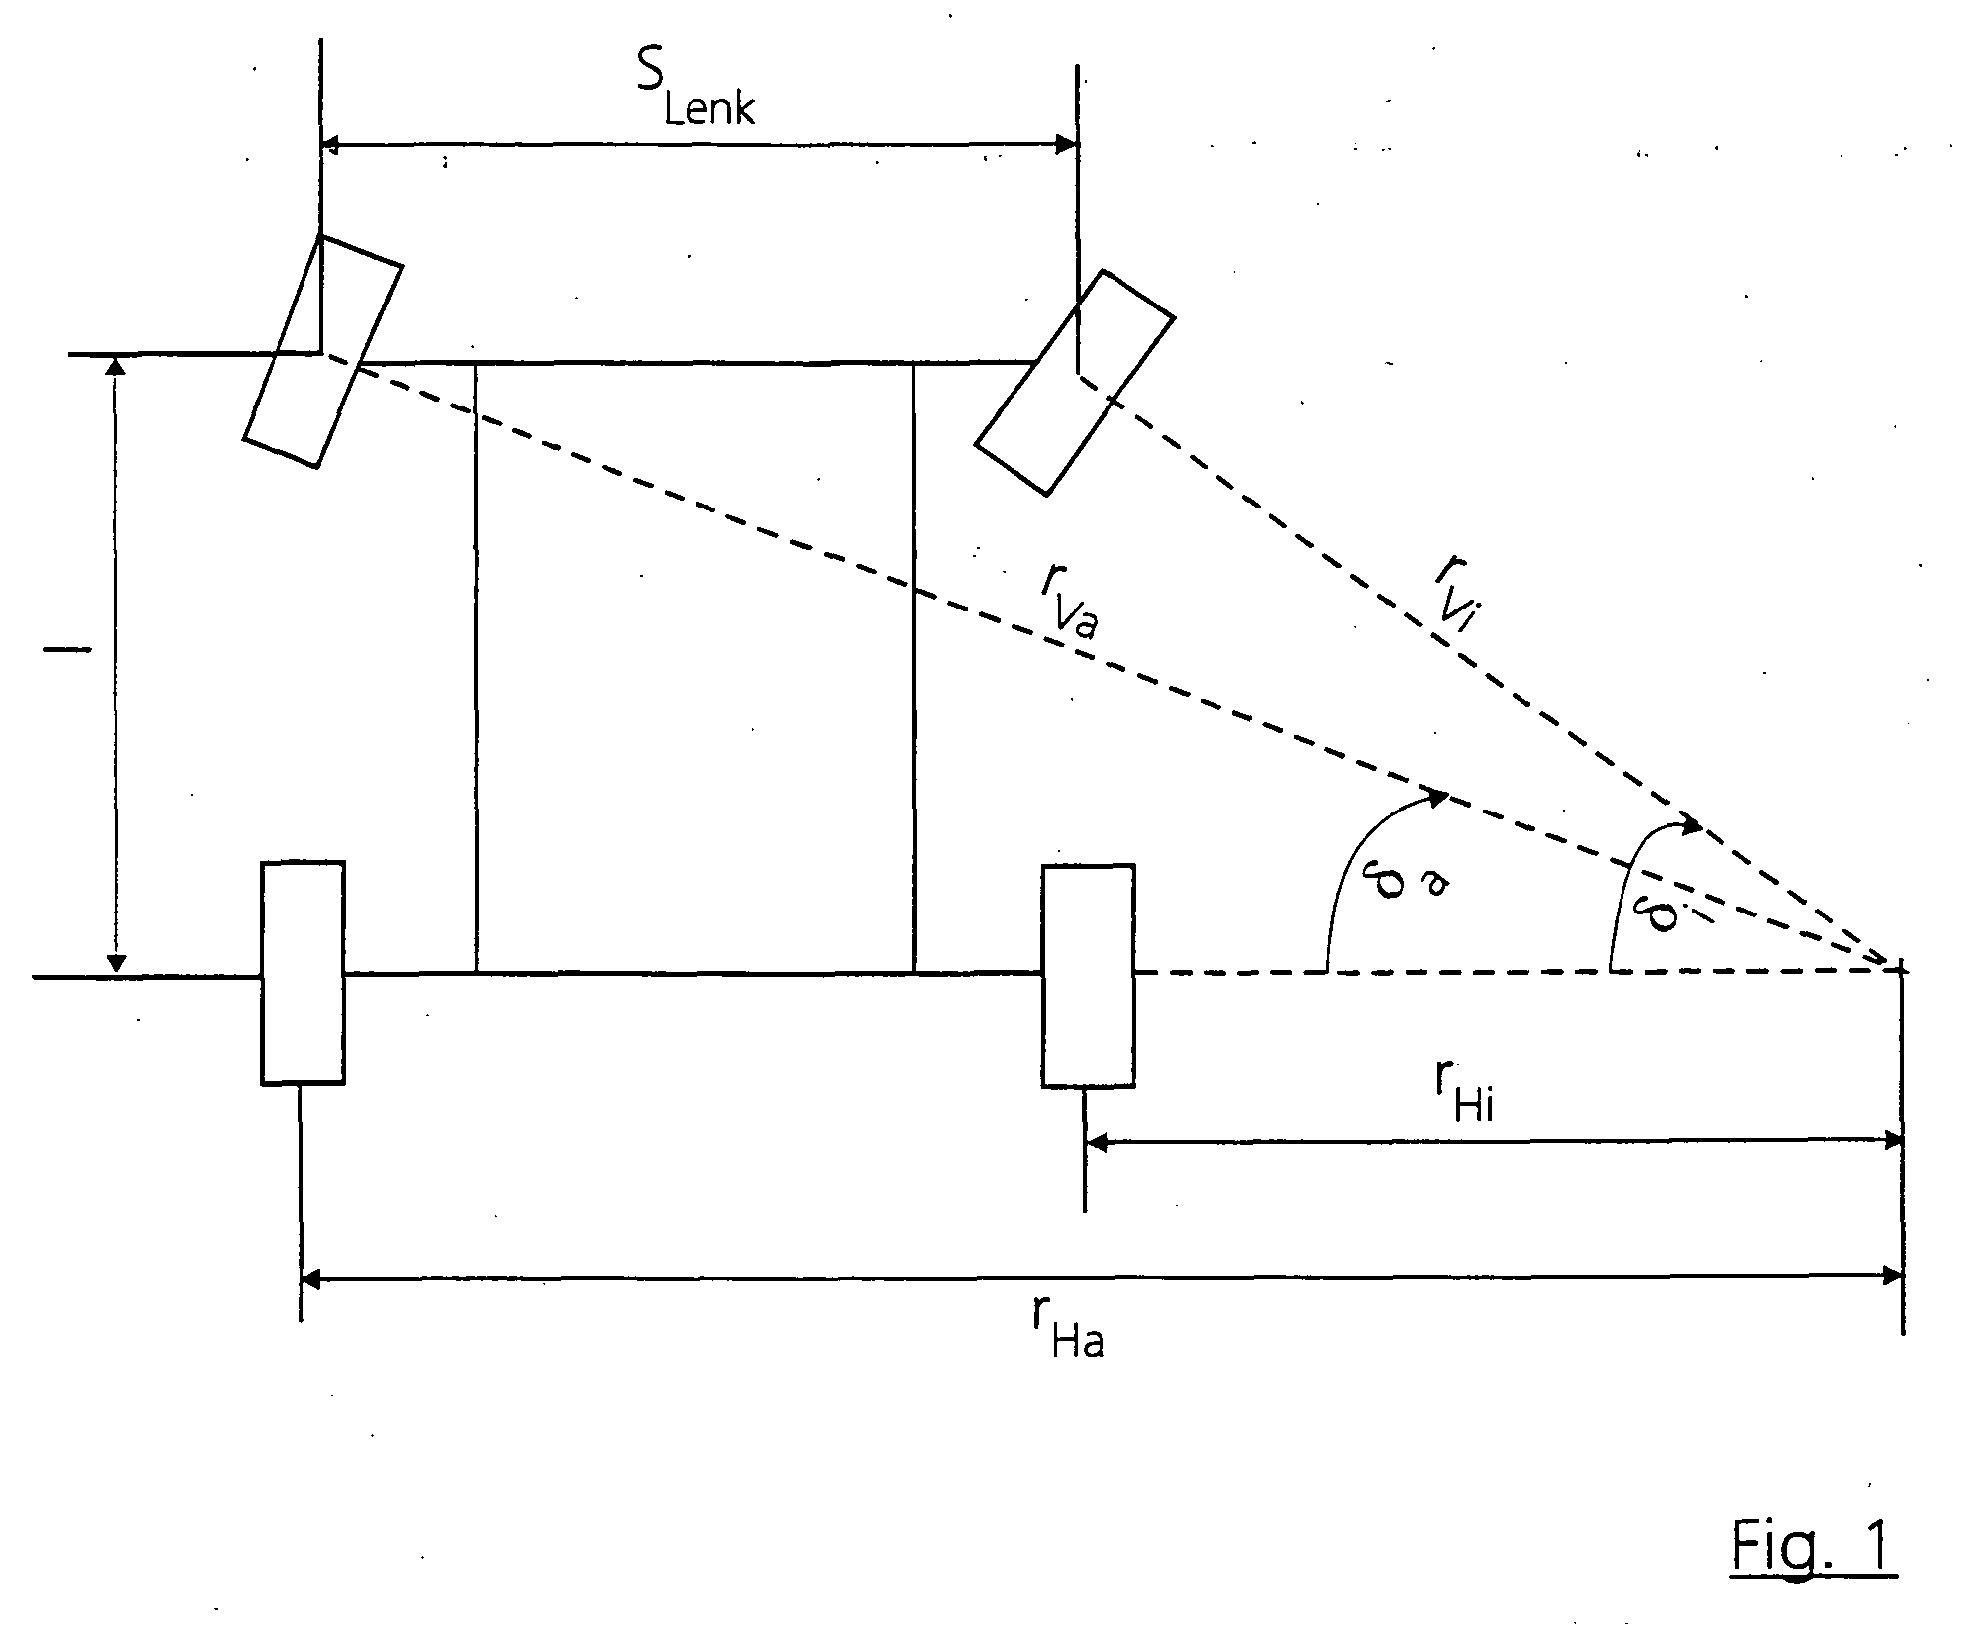
\includegraphics[width=(\textwidth/2)]{images/Ackermann.png}
    \caption{Achsschenkellenkung bei Starrachsen}
    \label{fig:Achsschenkellenkung bei Starrachsen}
\end{figure}
Beide Räder sollen bei Kurvenfahrt auf einer Kreisbahn mit gleichem Mittelpunkt rollen, dem Momentanpol der Bewegung. Bei der Drehschemellenkung ist das automatisch der Fall. Bei einer Einzelradlenkung muss das innere Rad, das näher am Mittelpunkt liegt und dem äußeren vorauseilt, stärker einlenken als das äußere. Bei der Achsschenkellenkung müssen die Räder unterschiedlich geschwenkt werden, das außen liegende weniger stark als das innen liegende. Das erreicht man mit der Bildung des sogenannten Lenktrapezes aus dem Achskörper, den beiden leicht nach innen weisenden Lenkhebeln an den Achsschenkeln und einer Spurstange, die kürzer als der Achskörper ist. Dadurch entstehen beim Schwenken der Räder ungleich lange wirksame Hebelarme, so dass sich die Verlängerungen aller Radachsen ungefähr im Kurvenmittelpunkt schneiden (Ackermann-Prinzip). Ein Hinweis auf ein richtig dimensioniertes Lenktrapez ist die Tatsache, dass sich die verlängerten Lenkhebel an den Achsschenkeln in Geradeausstellung in der Mitte der Hinterachse treffen (siehe oben in obiger Abbildung).\\

Wenn nach rechts gesteuert wird werden diese für den Winkel der beiden Räder verwendetet:
\begin{align}
    \textrm{Linkes Rad}& =\arctan^{-1}\left(\frac{\textrm{Achsenabstand}}{\textrm{KurvenRadius}+\frac{\textrm{RadAbstand}}{2}}\right)\\
    \textrm{Rechtes Rad}& =\arctan^{-1}\left(\frac{\textrm{Achsenabstand}}{\textrm{KurvenRadius}-\frac{\textrm{RadAbstand}}{2}}\right) 
\end{align}

%Wie wurde die Formel im Code umgesetzt?
Im ScrWheelcontroller Script wird der Ackermannwinkel berechnet wird. Der berechnete Ackermannwinkel wird an die vordernen beiden Räder weitergegeben. Die Räder werden zuvor in einer Liste hinzugefügt.
%Warum wurde es so umgesetzt?
Es brauchte ein Controller Script verwendet um die Struktur übersichtlicher zugestalten. Im Wheelscripts werden public bools angelegt die im Inpector dort wird fest gelegt um welches Rad es sich handelt.


\begin{lstlisting}
private void manuelSteering()
{
            
    if (steerInput > 0)
    {
        ackermannAngleLeft = Mathf.Rad2Deg * Mathf.Atan(wheelBase / (turnRadius + (rearTrack / 2))) * steerInput;
        ackermannAngleRight = Mathf.Rad2Deg * Mathf.Atan(wheelBase / (turnRadius - (rearTrack / 2))) * steerInput;
    }
    else if (steerInput < 0)
    {
        ackermannAngleLeft = Mathf.Rad2Deg * Mathf.Atan(wheelBase / (turnRadius - (rearTrack / 2))) * steerInput;
        ackermannAngleRight = Mathf.Rad2Deg * Mathf.Atan(wheelBase / (turnRadius + (rearTrack / 2))) * steerInput;
    }
    else
    {
        ackermannAngleLeft = 0;
        ackermannAngleRight = 0;
    }
}    
\end{lstlisting}


\subsection{Beschleunigung}
%wie funktioniert die Beschleunigung?
%Diese muss im späteren verlauf verändert werden vorübergehen geht es in ordnung
%Die beschreibung am besten so durch führen wie es in dem einem Youtube video gezeigt wurde
\subsection{Steuerung}
%Wie wird die Spurr gezeichnet?

%Wie wird gesteuert?
Die Publicvariablen sollen verändert werden.